\section{Introduction to Neural Networks}

\subsection{Artificial Neural Networks}
Artificial Neural Networks (ANN) \cite{haykin2004comprehensive} are bionics network structures inspired by the performance of the human brain. Its basic idea is to build complex network structure by connecting a large number of simple neurons, which allows signals to be transmitted from one neuron to another. Signals are amplified or attenuated by activating different neurons and adding weights.

\subsubsection{Fundamental of ANN}
Figure 1 shows a traditional ANN structure:

\begin{figure}[]
\centering
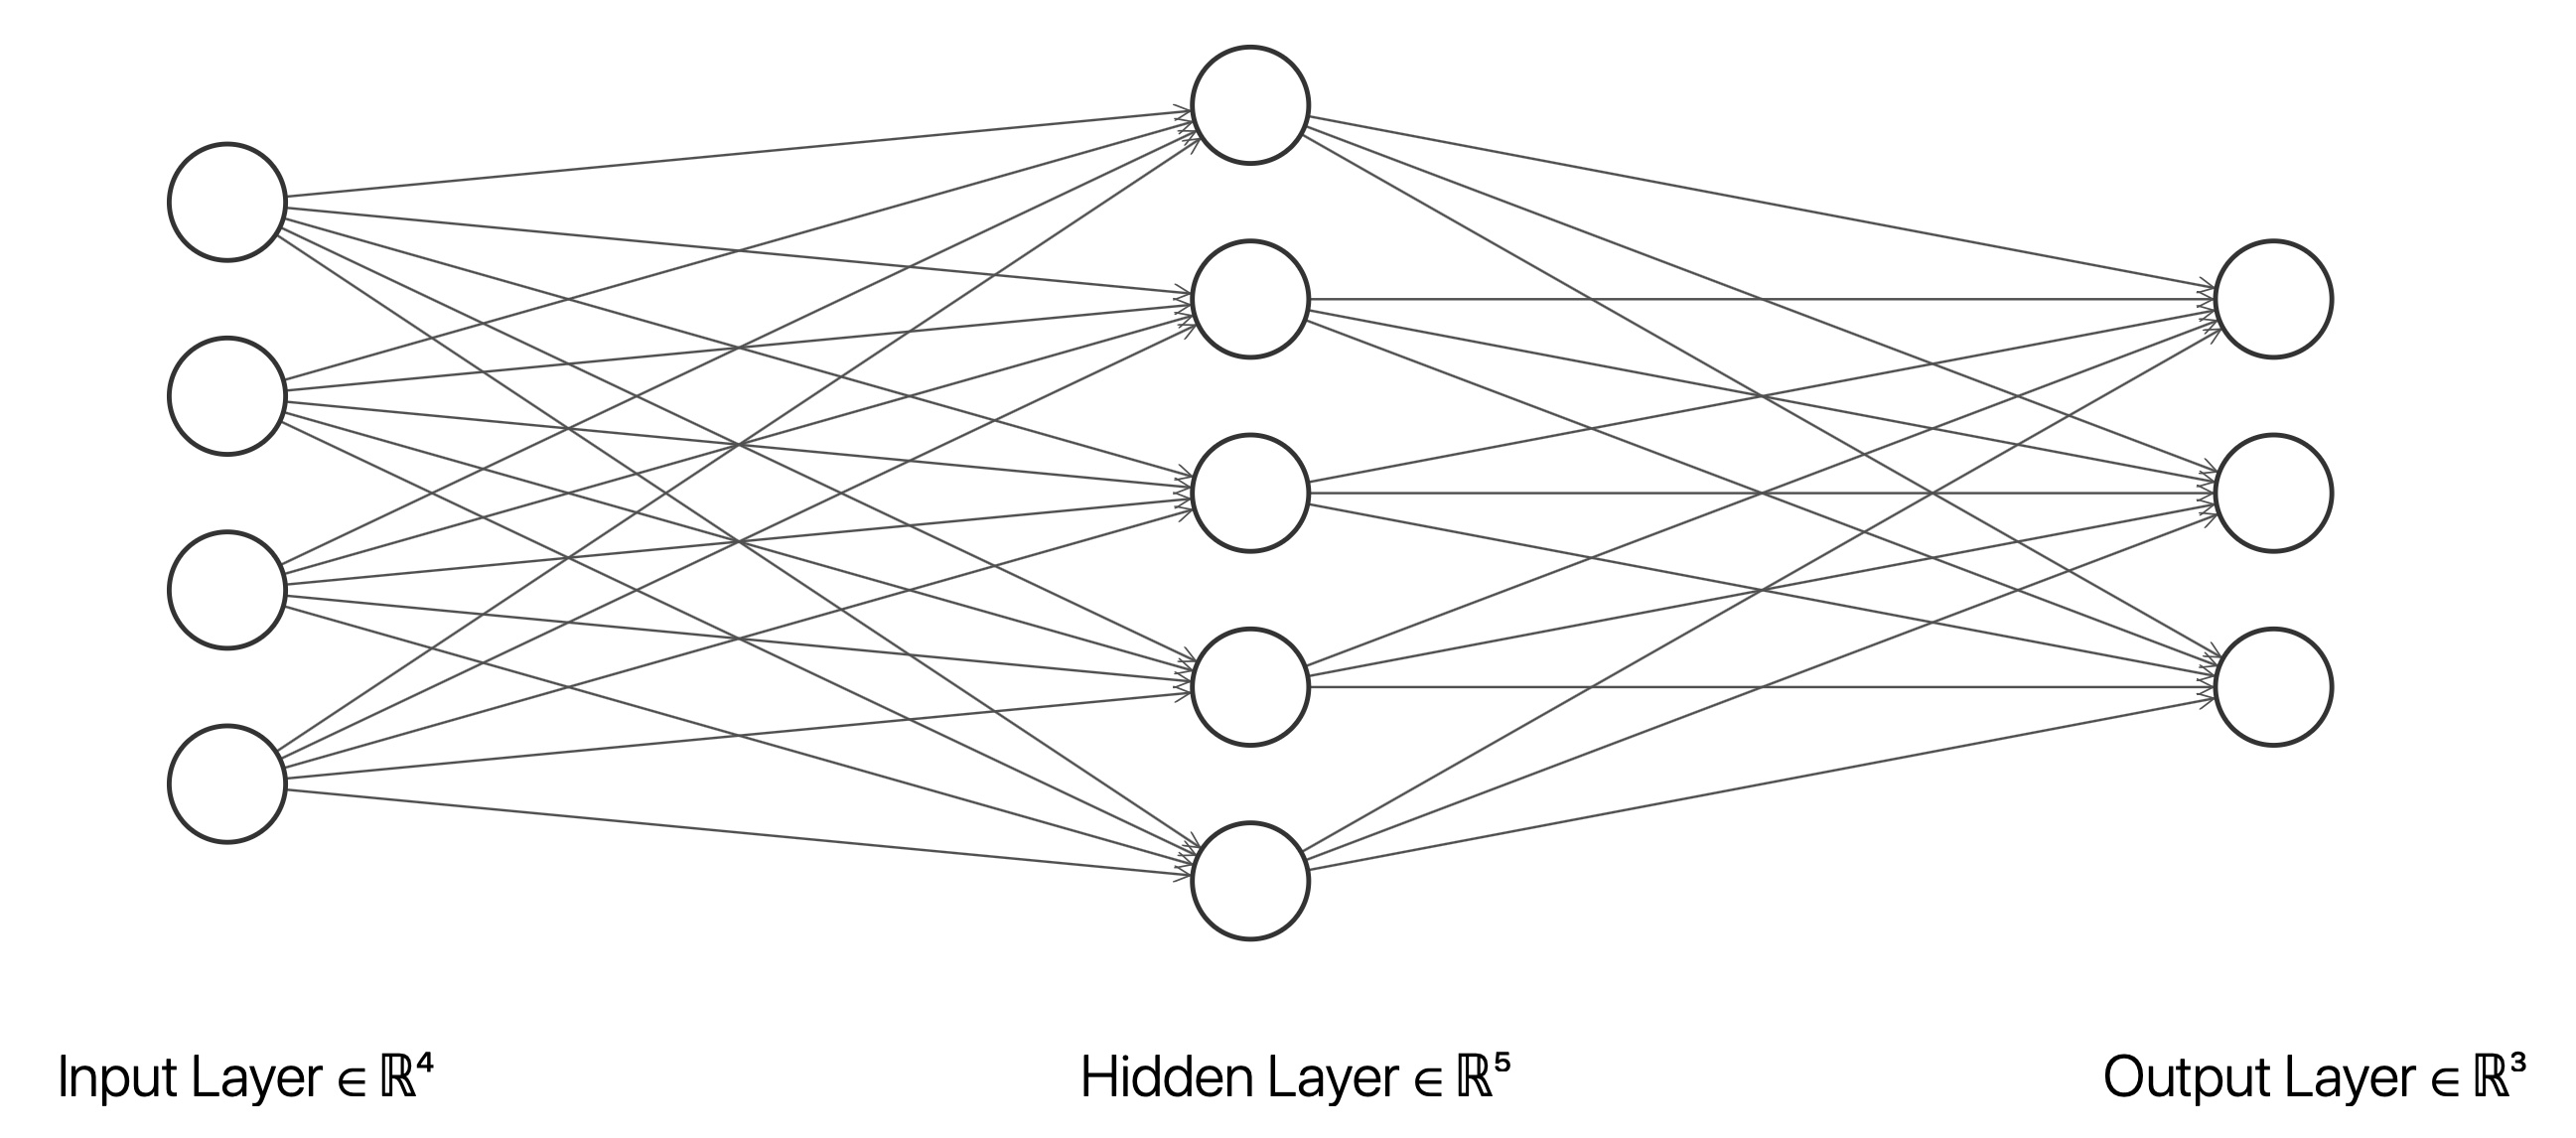
\includegraphics[width=0.59\textwidth]{figures/ANN_sample.jpg}
\caption{Simple fully connected neural network}
\label{fig:B-B1}
\end{figure}

\begin{itemize}
\item Input layer: contains several neurons and receives multi-dimension input signals.
\item Output layer: contains several neurons and produces multi-dimension output signals.
\item Hidden layer: contains several layers and each layer contains several neurons.
\end{itemize}
When signals are fed to certain neuron, they are multiplied by weights of the connections and added together. Then the weighted sum is passed through an activation function to produce the output. Some commonly used activation functions are listed in table 1.

%\renewcommand\arraystretch{4}
\begin{table}[]
\centering
\begin{tabular}{|c|c|c|}
\hline
\textbf{Activation Function}  & \textbf{Equation} & \textbf{Plot} \\ \hline
Sigmoid Function                 & $f(x) = \frac{1}{1+e^{-x}}$
& \begin{minipage}[b]{0.25\columnwidth}
    \centering
	\raisebox{-.5\height}{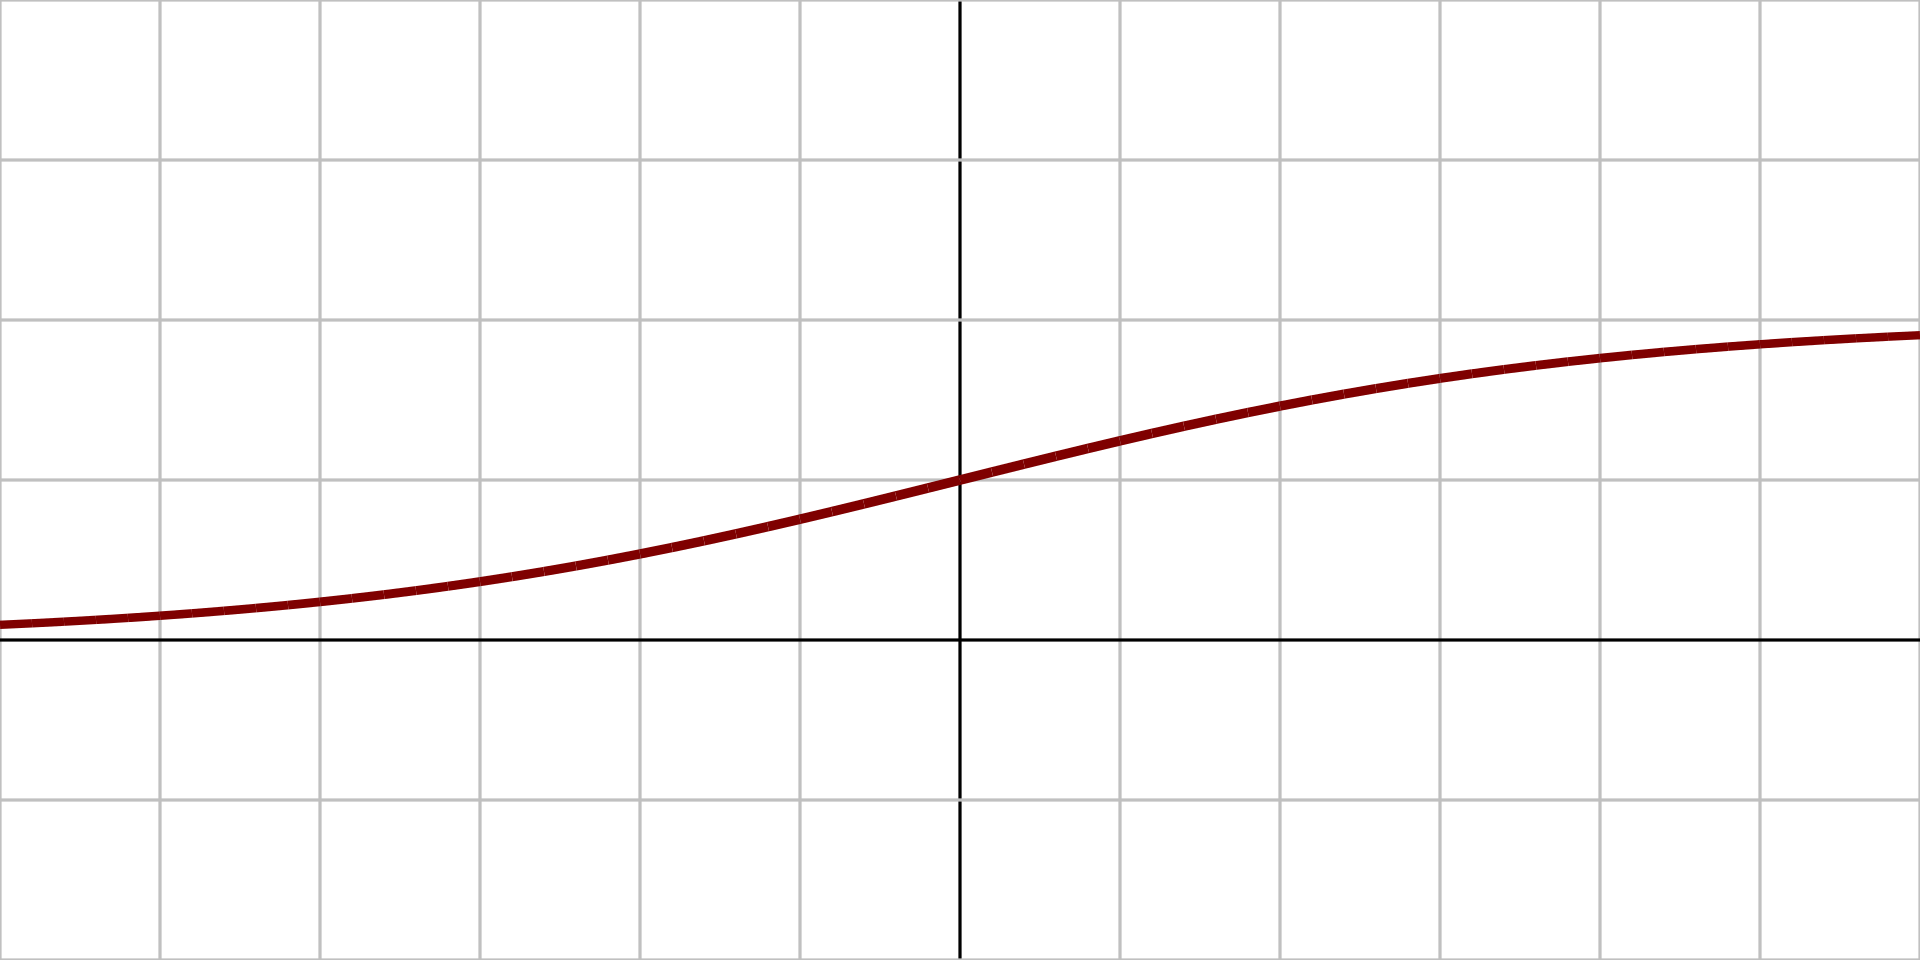
\includegraphics[width=\linewidth]{figures/sigmoid.png}}
	\end{minipage}\\ \hline
Hyperbolic Tangent Function      & $f(x) = \frac{e^x-e^{-x}}{e^x+e^{-x}}$ 
& \begin{minipage}[b]{0.25\columnwidth}
    \centering
	\raisebox{-.5\height}{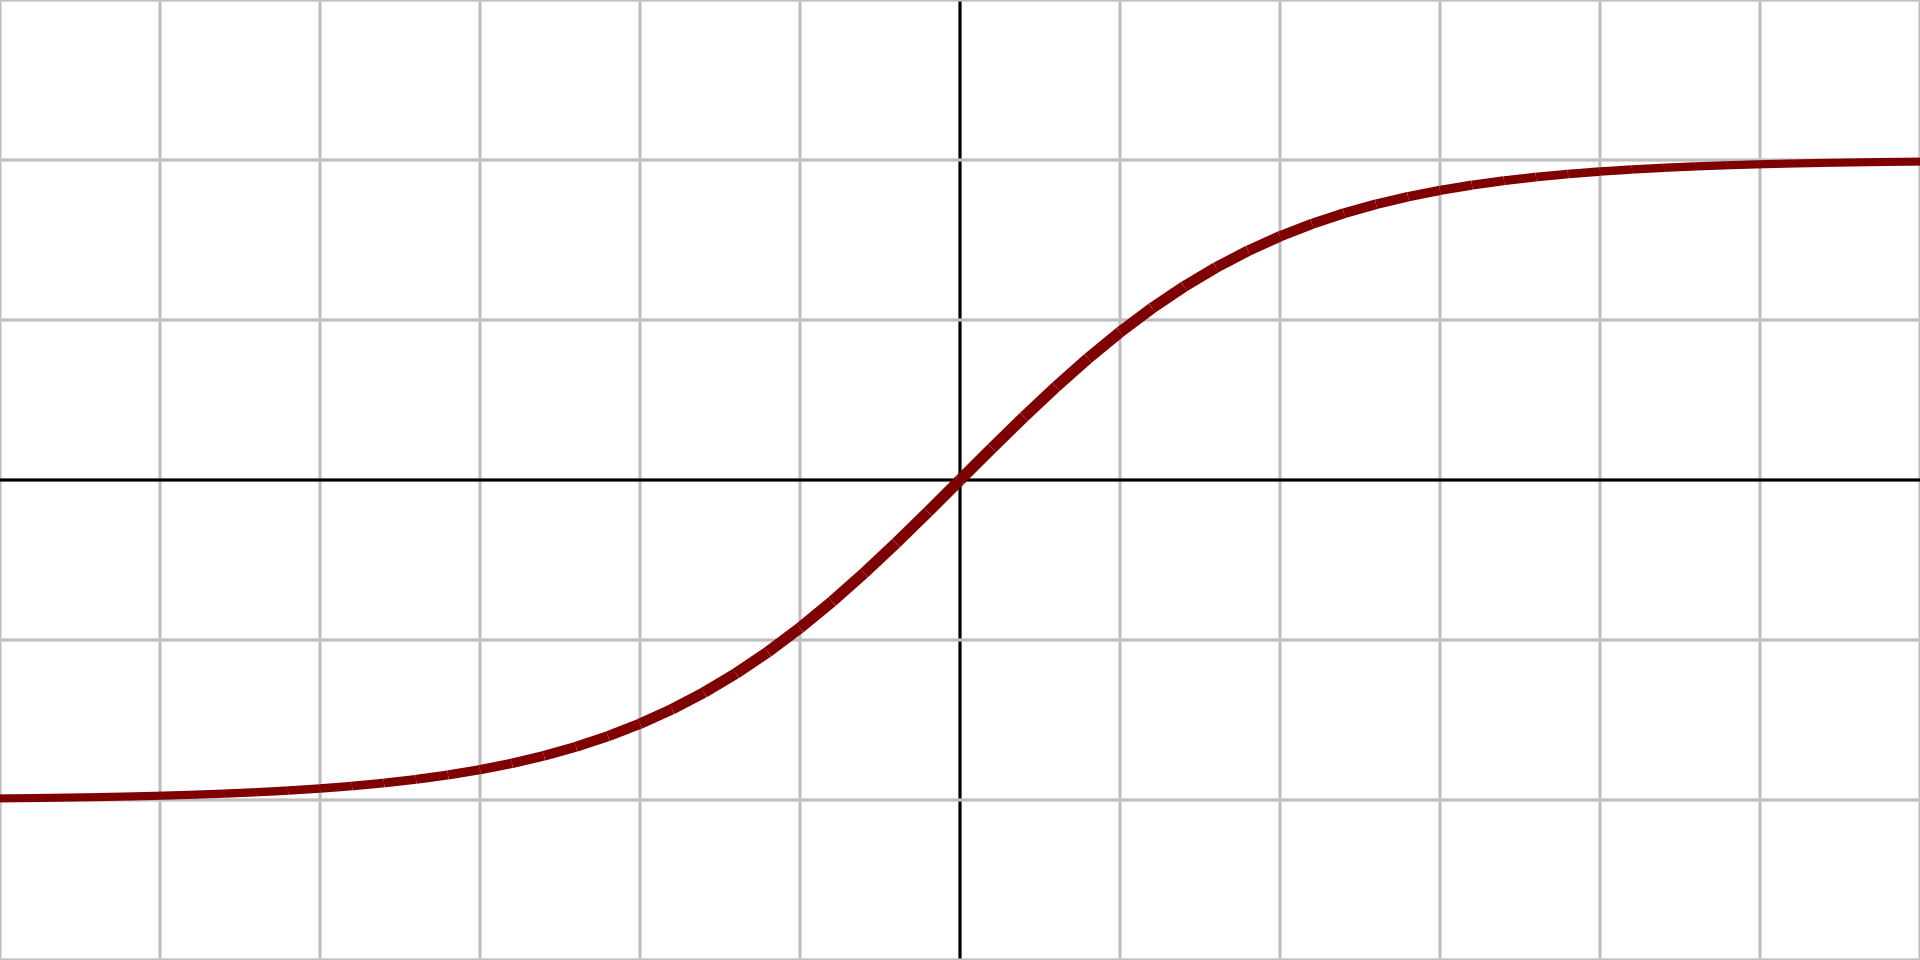
\includegraphics[width=\linewidth]{figures/tanh.png}}
	\end{minipage}\\ \hline
Rectified Linear Unit Function    & $ f(x)=\left\{
\begin{aligned}
x = & 0 & for \ x \leq 0\\
y = & x & for \ x > 0
\end{aligned}
\right.
$
& \begin{minipage}[b]{0.25\columnwidth}
    \centering
	\raisebox{-.5\height}{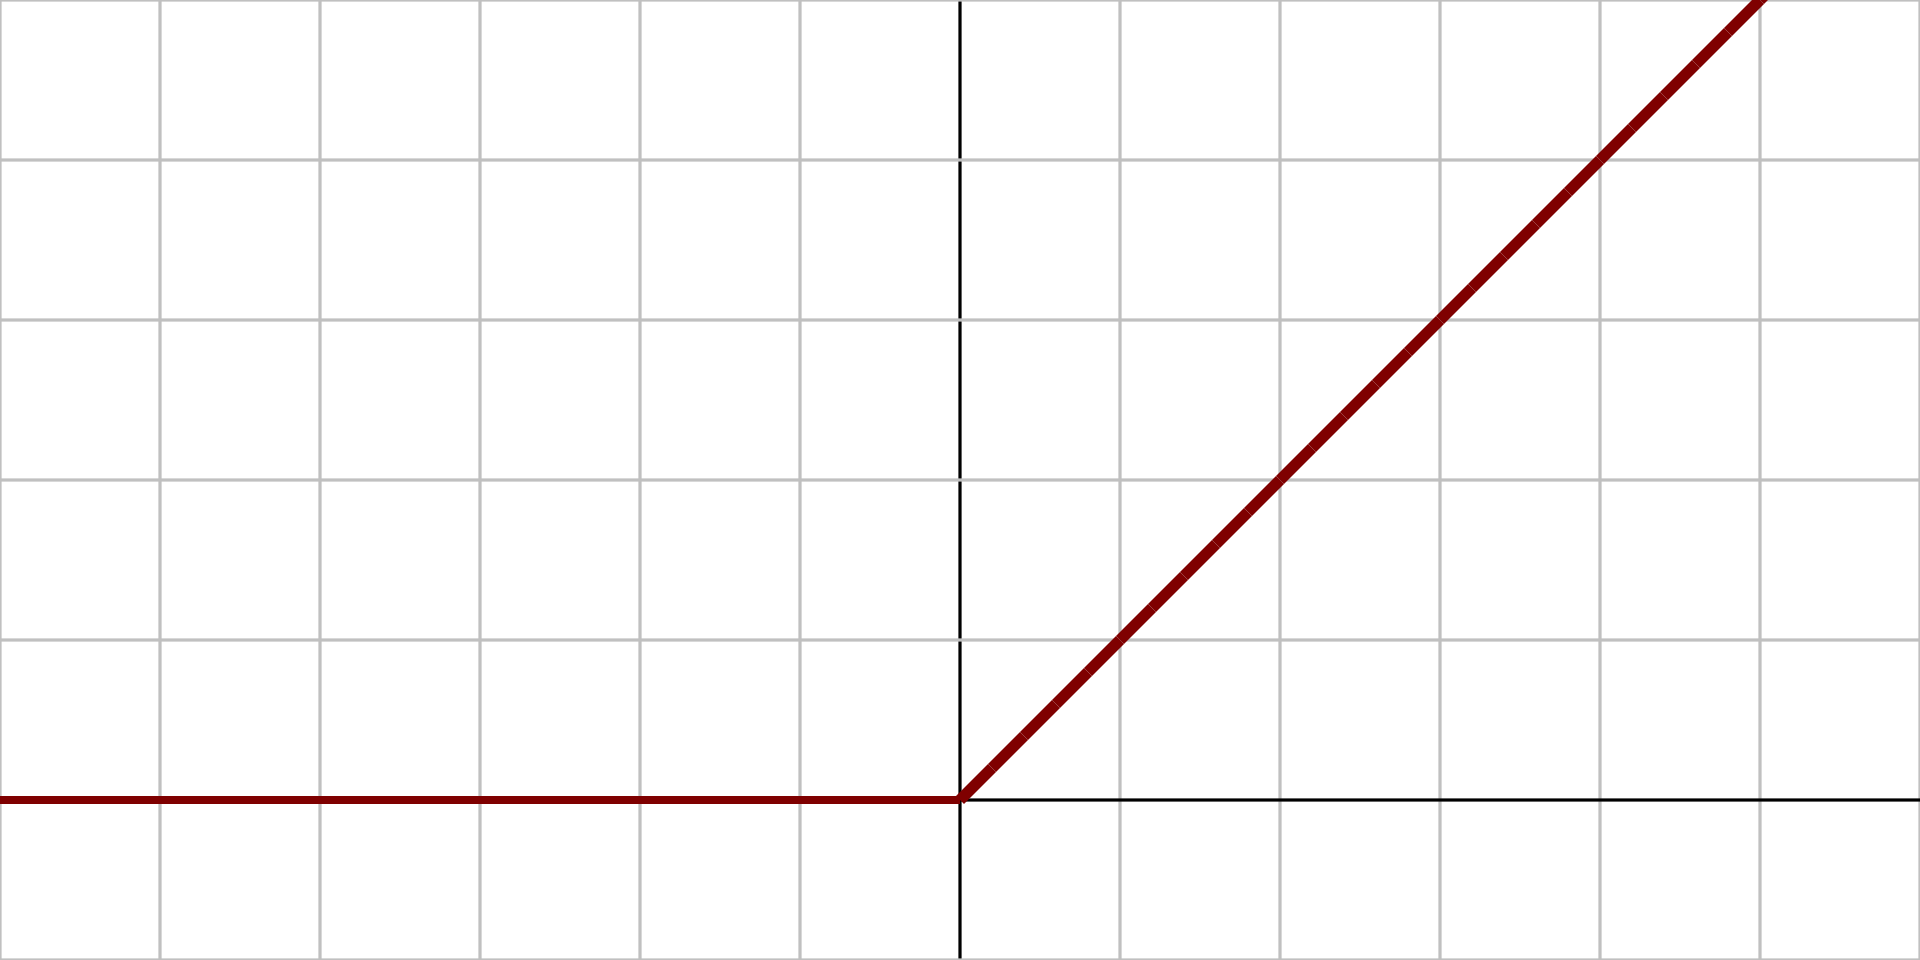
\includegraphics[width=\linewidth]{figures/rectified_linear.png}}
	\end{minipage}\\ \hline
Leaky Linear Unit Function       & $ f(x)=\left\{
\begin{aligned}
x = & 0.01x & for \ x < 0\\
y = & x & for \ x \geq 0
\end{aligned}
\right.
$        
& \begin{minipage}[b]{0.25\columnwidth}
    \centering
	\raisebox{-.5\height}{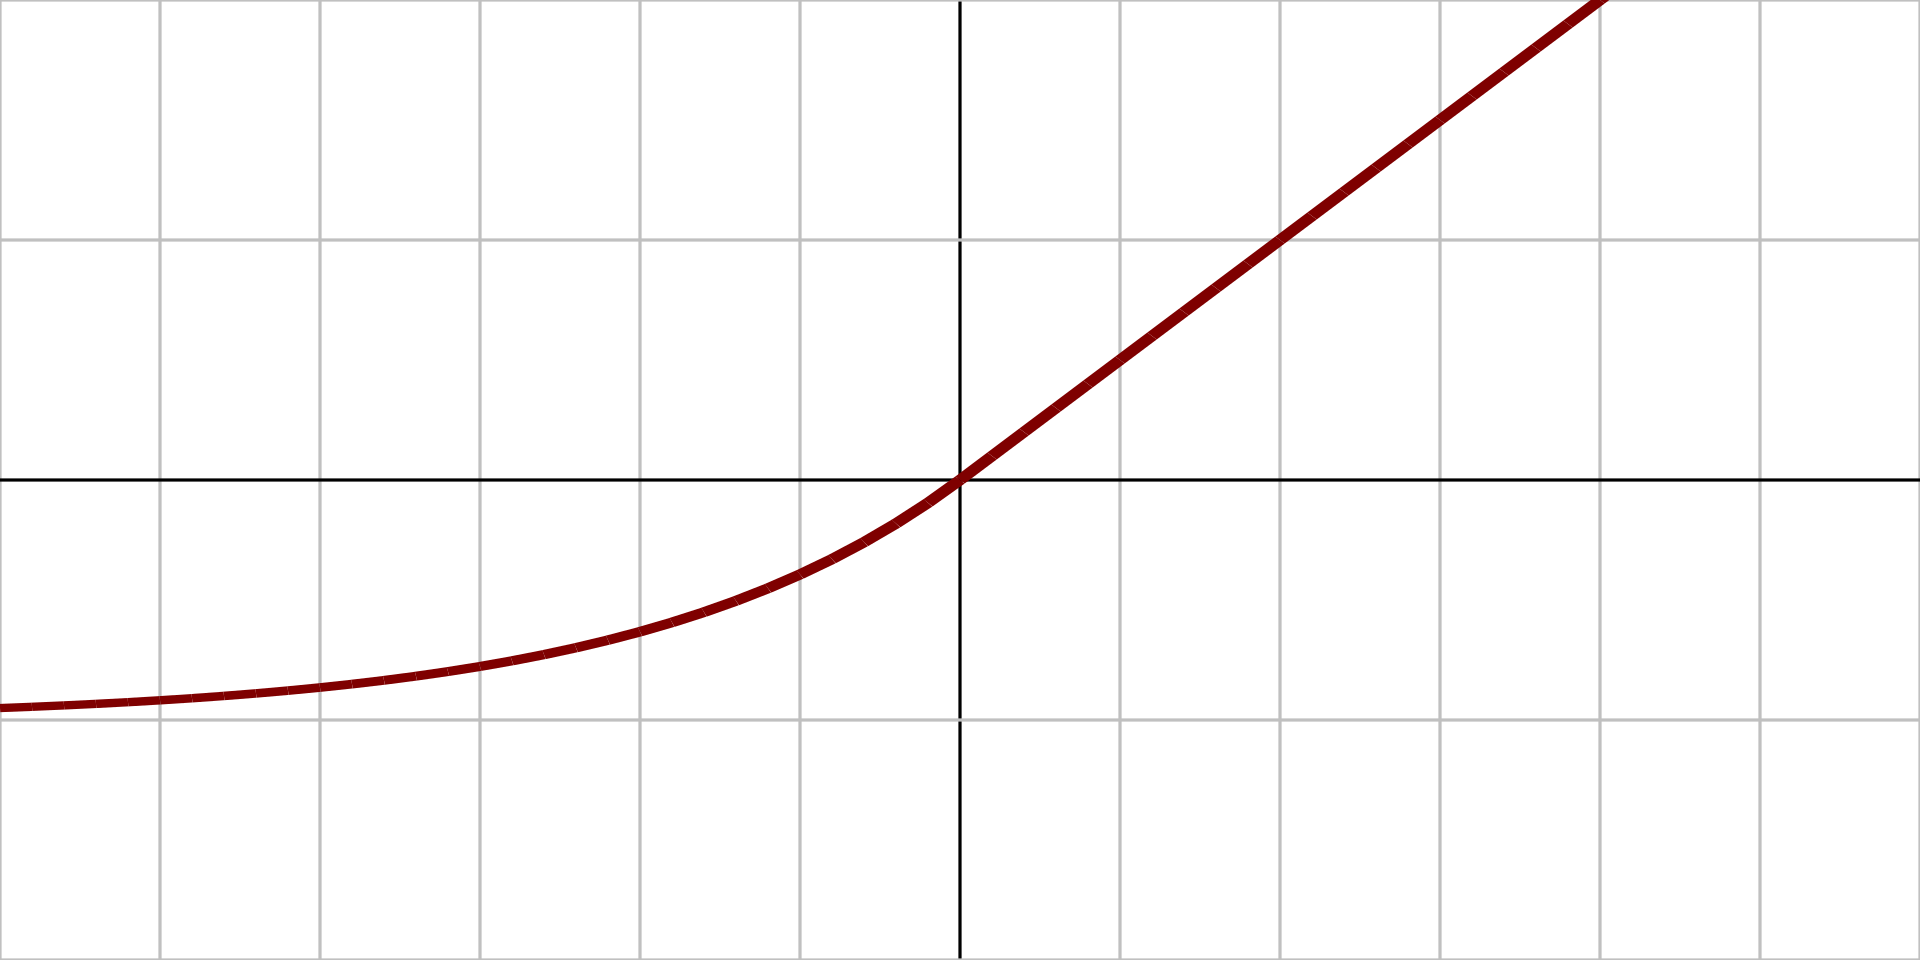
\includegraphics[width=\linewidth]{figures/Activation_elu.png}}
	\end{minipage}\\ \hline
Exponential Linear Unit Function & $ f(x)=\left\{
\begin{aligned}
x = & \alpha x & for \ x < 0\\
y = & x & for \ x \geq 0
\end{aligned}
\right.
$
& \begin{minipage}[b]{0.25\columnwidth}
    \centering
	\raisebox{-.5\height}{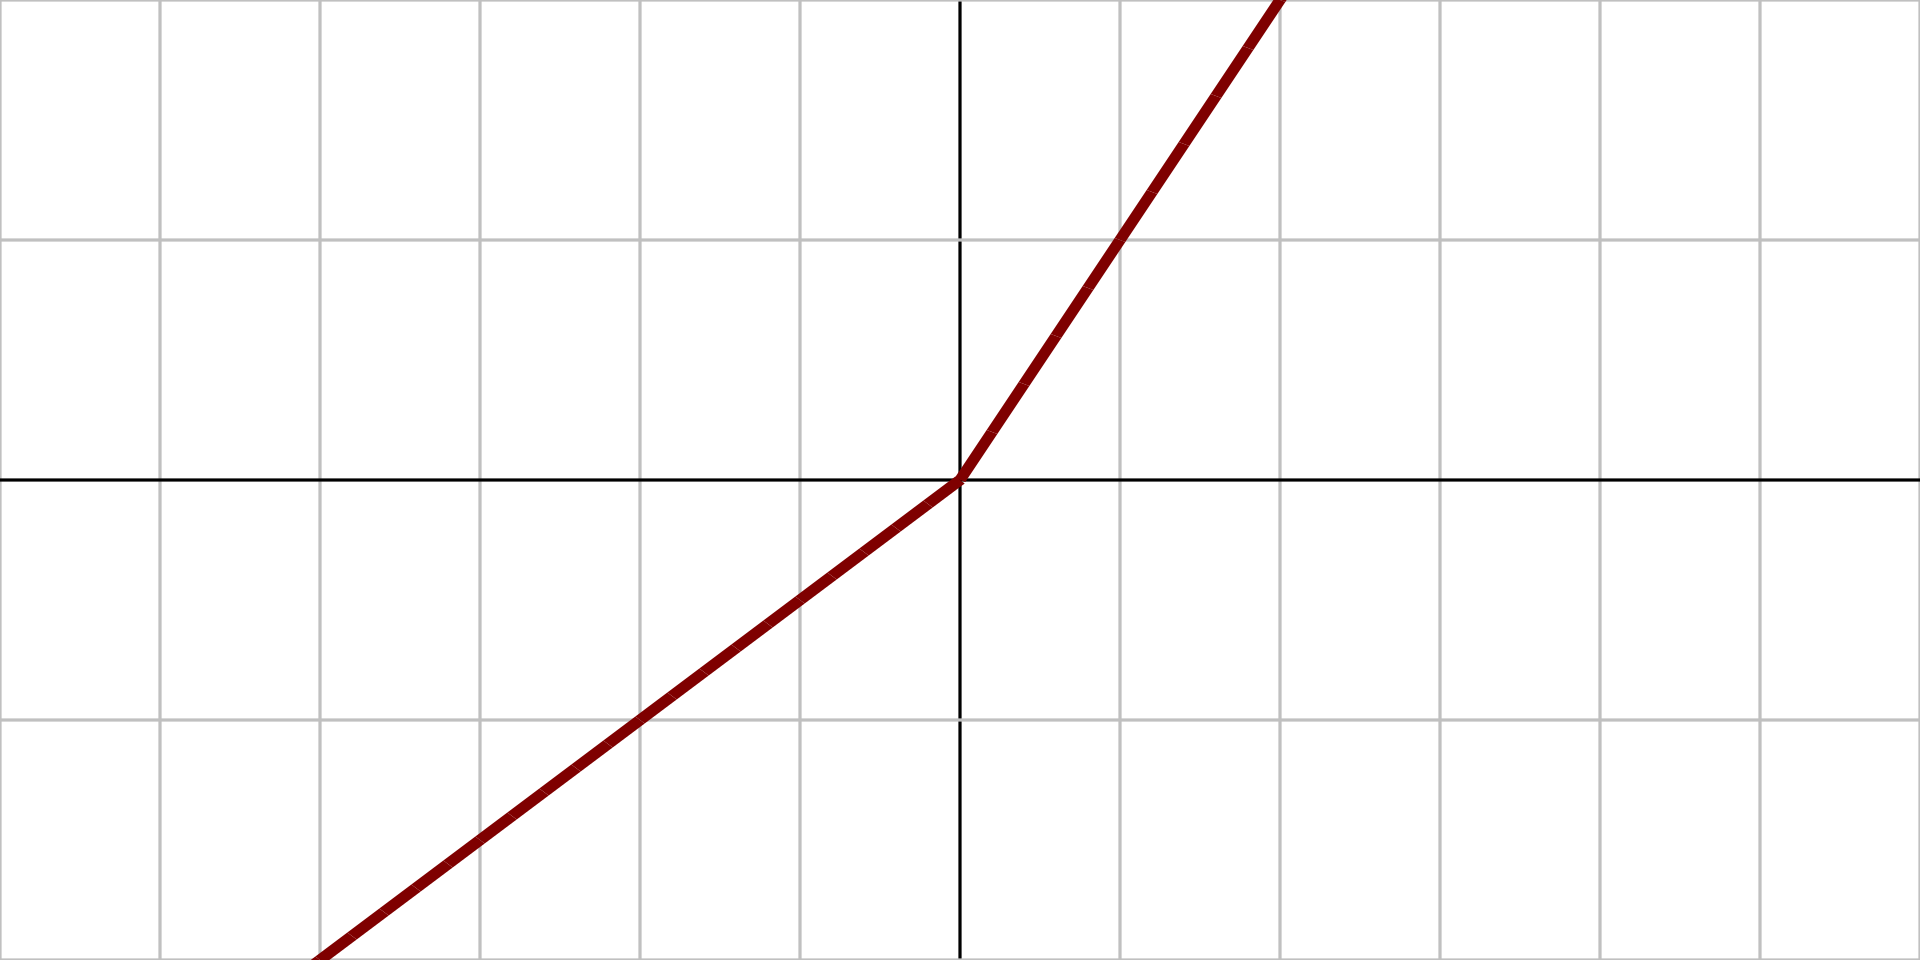
\includegraphics[width=\linewidth]{figures/prelu.png}}
	\end{minipage}\\ \hline
\end{tabular}
\caption{Common activation functions}
\end{table}

Number of layers, number of neurons, connection between neurons and activation functions are main factors that determine a network's performance. We can build different ANN by using different choices of these factors. An ANN model's performance can be quite different when the model is applied on different kinds of input signals. There is no universal ANN model that performs well on all kinds of signals.

\subsubsection{Shortcomings of traditional ANN}

In traditional fully connected neural network, signals are transmitted from input layer to the output layer in sequence. And there's no interaction between neurons in the same layer. Here comes a problem that the output signal only depends on the input signal, and has nothing to do with the order of the input signal. Moreover, the neuron itself does not have the ability to store information, and the entire network does not have the “memory” ability. When the input signal is time-related, for example a time series, the performance of traditional neural network structure 
will be very poor.

\subsection{Recurrent Neural Networks}
As was stated in previous section, traditional neural networks don't perform well on time-related data. Recurrent neural networks (RNN) address this issue. They are special networks with loops in them, allowing information to persist.

\subsubsection{Structure of RNN}

\begin{figure}[]
\centering
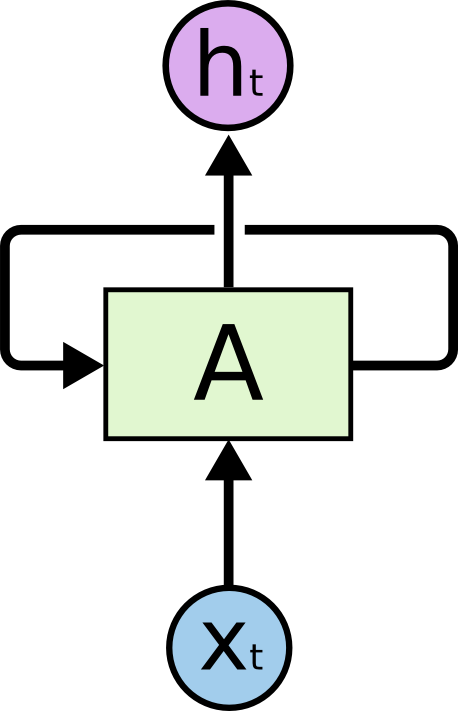
\includegraphics[width=0.15\textwidth]{figures/RNN-rolled.png}
\caption{Recurrent Neural Networks}
\label{fig:B-B1}
\end{figure}

Figure 2 shows the compact structure of RNN, where $x_t$ is input signal, $h_t$ is output signal and A is a chunk of neural networks which allows information to be passed from one step of the network to the next. To make it clear, a RNN can be regard as multiple copies of the same network, each passing a message to a successor.

\subsubsection{Shortcomings of RNN}
One of the advantages of RNNs is that they might be able to connect previous information to the present task. However, when the gap between the relevant information and the point where it is needed is very large, for example a long time series data, RNNs become unable to learn their relationship.

\begin{figure}[]
\centering
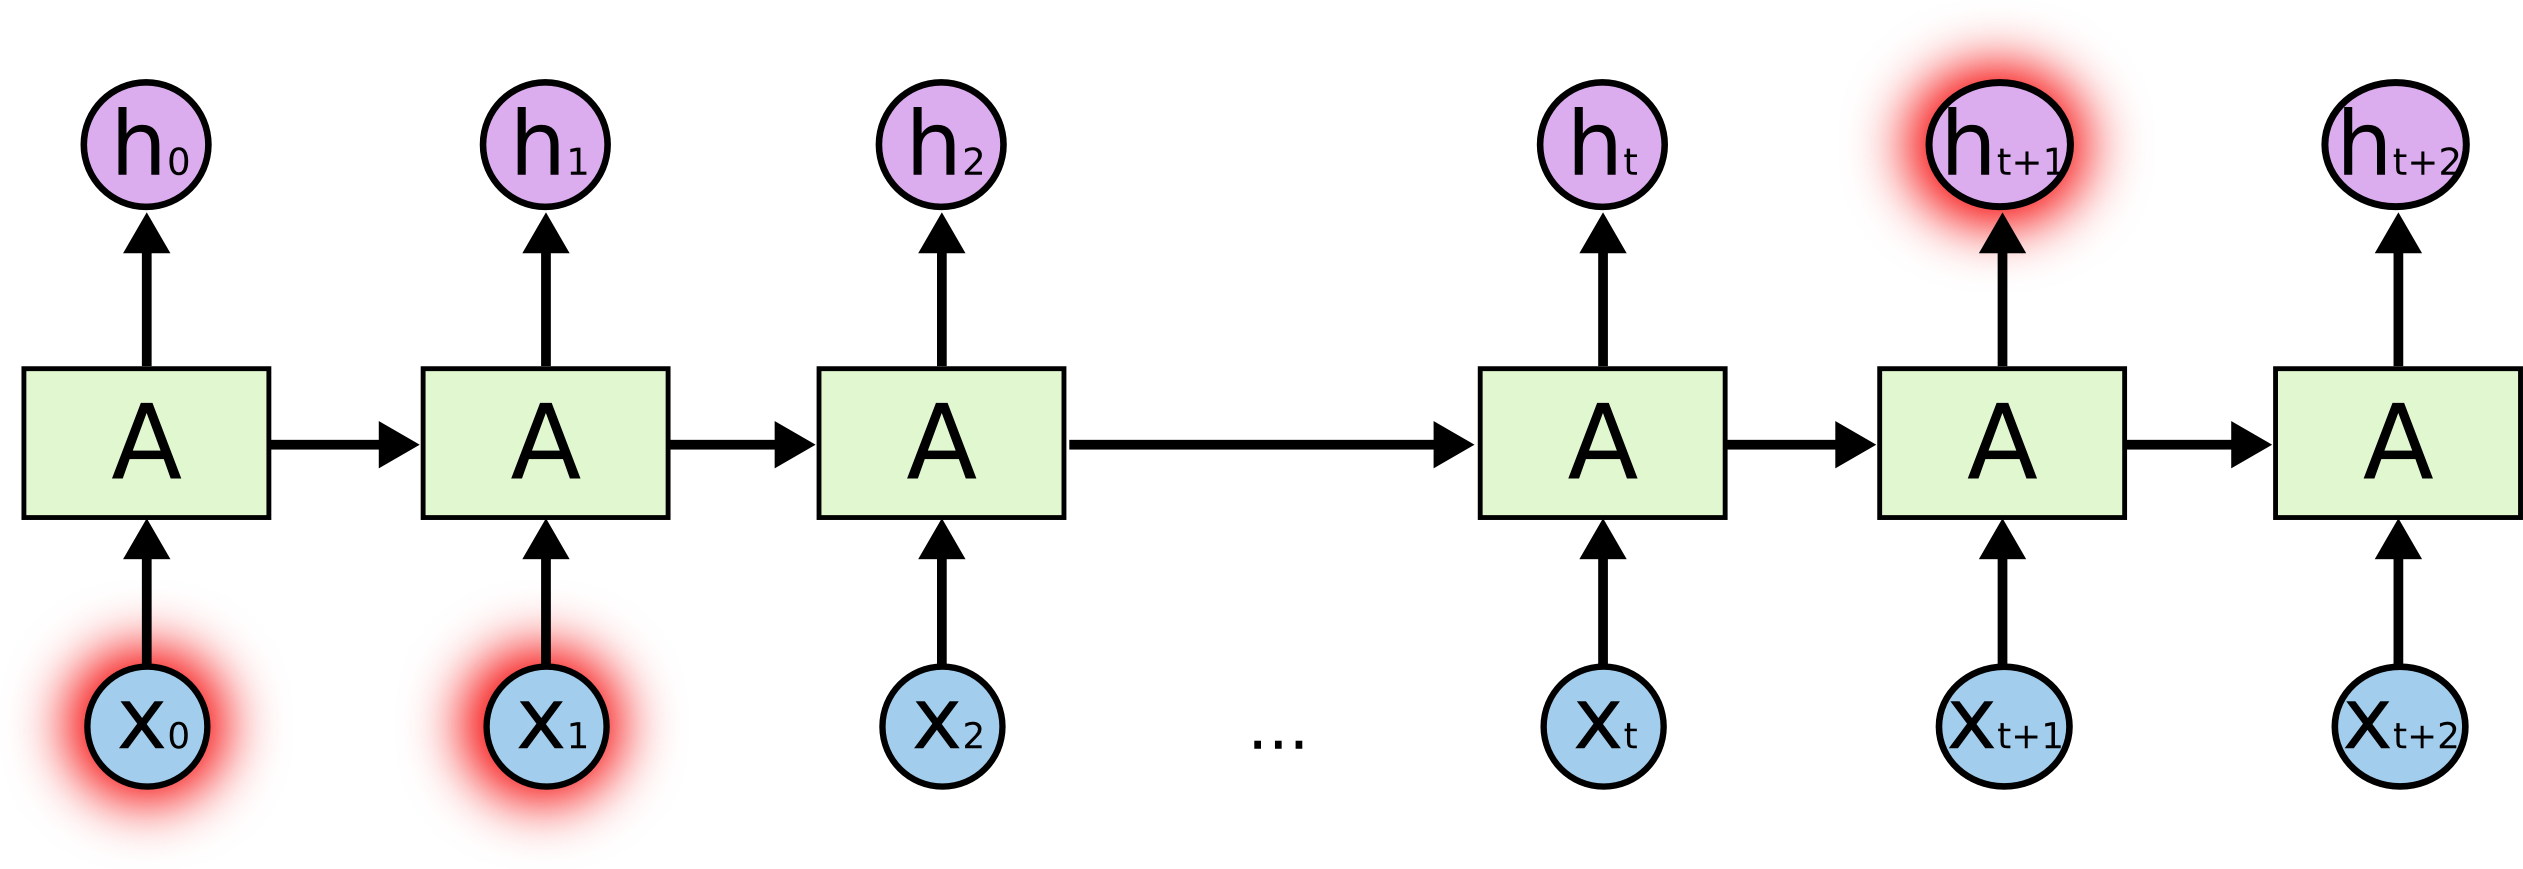
\includegraphics[width=0.6\textwidth]{figures/RNN-longtermdependencies.png}
\caption{The problem of long-term dependencies}
\label{fig:B-B1}
\end{figure}

\subsubsection{Long Short Term Memory networks}
Long Short Term Memory networks (LSTM) are a special type of RNN, which are capable of learning long-term dependencies. They were invented in 1997, and were developed and popularized by many people in following work. LSTM networks have same chain like structure as RNN, but the repeating module has a different structure. Repeating module in RNN only has a single neural network layer while there are four hidden layers which interact with each other in very special way in the repeating module of LSTM. Detailed introduction are shown in Appendix A.

\begin{figure}[]
\centering
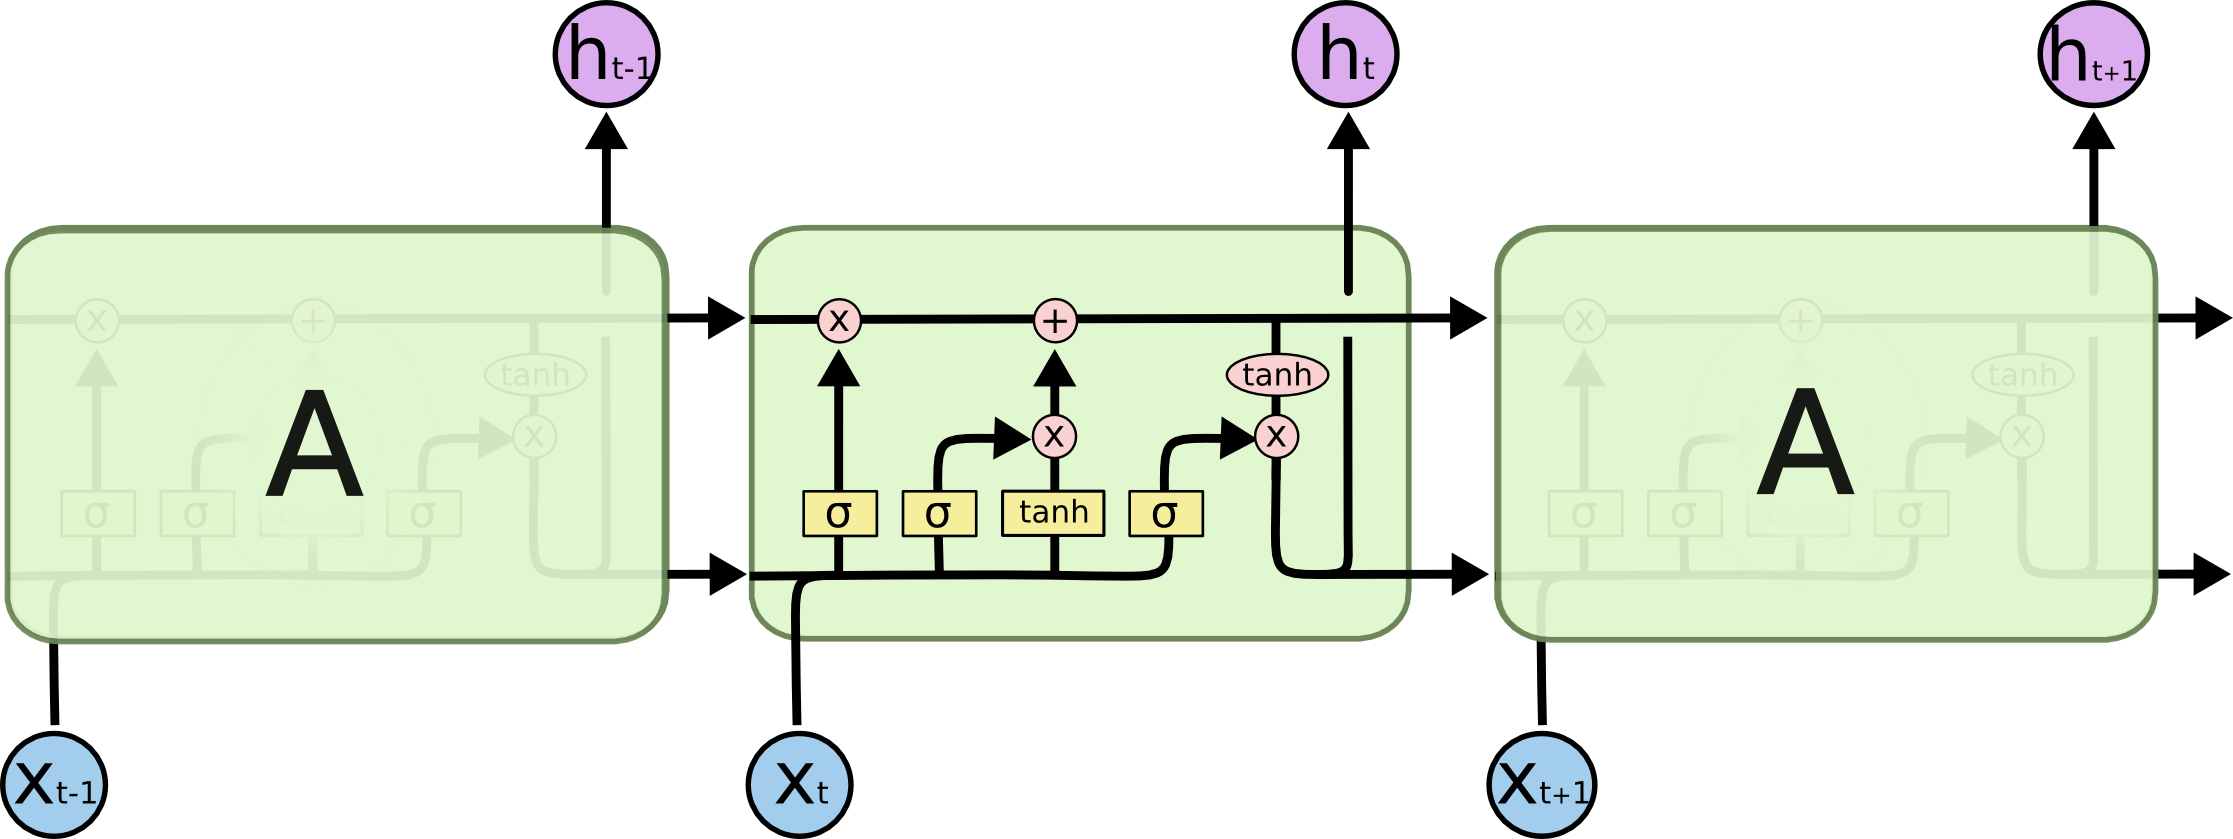
\includegraphics[width=0.6\textwidth]{figures/LSTM.png}
\caption{Structure of LSTM}
\label{fig:B-B1}
\end{figure}

\subsubsection{Conclusion}

In this section, the basic concepts required to develop a neural network models and the comparison between traditional ANN and LSTM has been introduced. The LSTM model is more capable of dealing with time series data which means it is a suitable method for this project.

\section{Overview of SCADA data}

\subsection{Data Acquisition}
All available SCADA parameters compiled in a typical wind turbine are presented in table 2.

\renewcommand\arraystretch{1.2}
\begin{table}[]
\centering
\begin{tabular}{|c|c|}
\hline
\textbf{Categories}          & \textbf{Variable name}         \\ \hline
\multirow{2}{*}{Environment} & Ambient temperature            \\ \cline{2-2} 
                             & Wind speed                     \\ \hline
\multirow{12}{*}{Status}     & Current                        \\ \cline{2-2} 
                             & Energy Export                  \\ \cline{2-2} 
                             & Gear oil temperature           \\ \cline{2-2} 
                             & Generator RPM                  \\ \cline{2-2} 
                             & Generator temperature          \\ \cline{2-2} 
                             & Grid Frequency                 \\ \cline{2-2} 
                             & High speed bearing temperature \\ \cline{2-2} 
                             & Nacele position                \\ \cline{2-2} 
                             & Power                          \\ \cline{2-2} 
                             & Reactive power                 \\ \cline{2-2} 
                             & Rotor speed                    \\ \cline{2-2} 
                             & Voltage                        \\ \hline
\end{tabular}
\caption{Available SCADA parameters}
\end{table}

\subsection{Data Visualization}
Before further transformation of data set, visualization techniques are used to extract the main characteristics and trends. Pandas library provides simple method to visualize the correlation between parameters. A correlation matrix of the selected variables was shown in figure 5 and the plots in the diagonal are density plots of each of the variables.

\begin{figure}[]
\centering
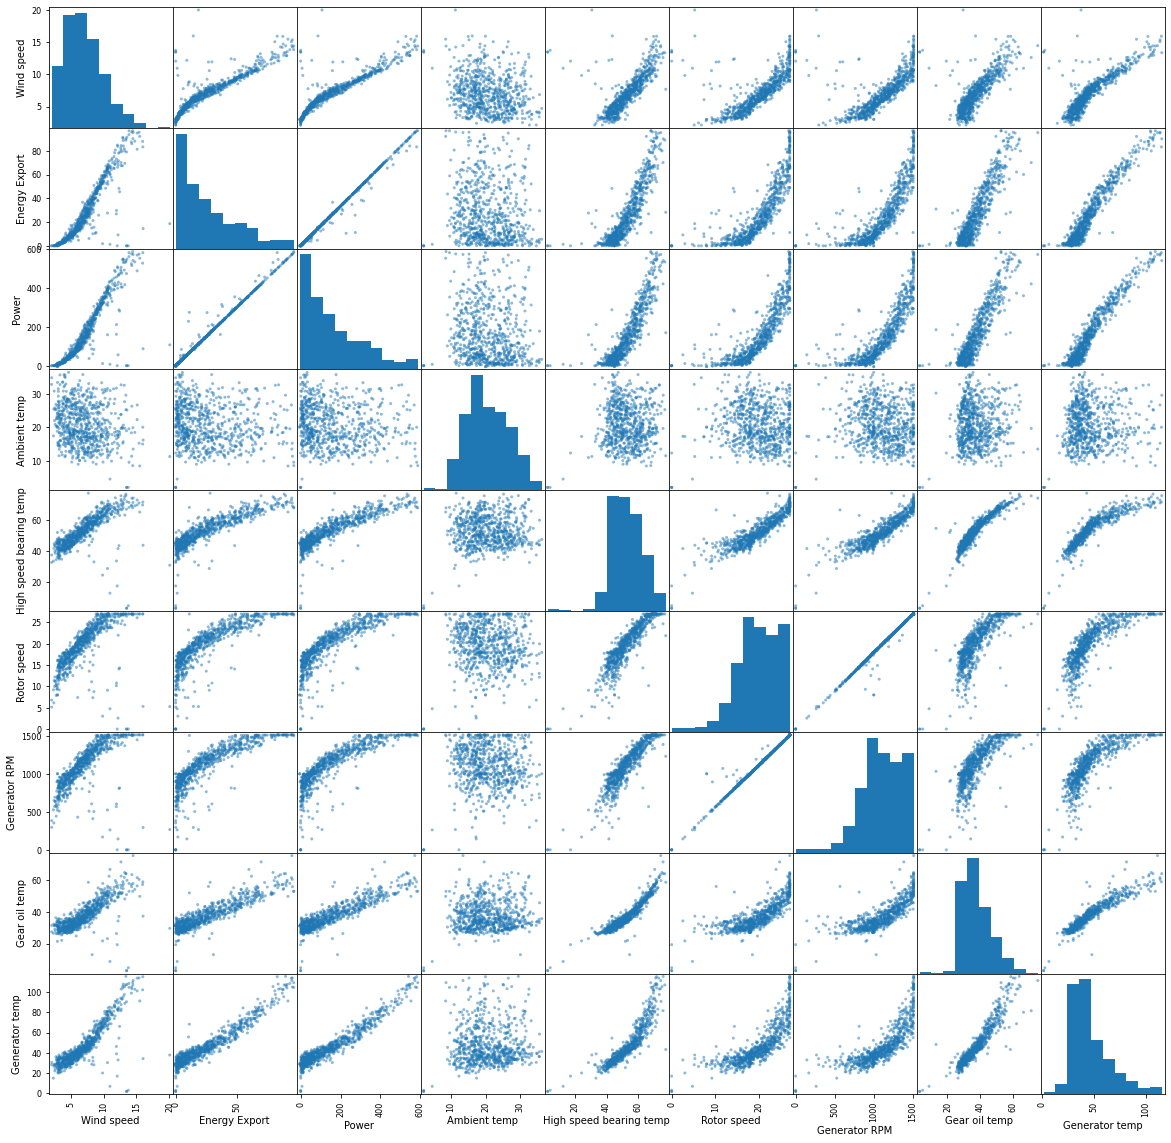
\includegraphics[width=0.9\textwidth]{figures/correlation_matrix.png}
\caption{Correlation matrix of the studied variables}
\label{fig:B-B1}
\end{figure}

If one variable presents a linear correlation with the other variable, one of them can be simply dropped since it doesn't provide any additional information in the model.

\subsection{Underlying Information of Data}
There are two different ways of understanding the SCADA data. One is to regard the data as a continuous time series, the other one is to regard them a several discrete data point. Both way make sense, but different understandings lead to different models.

For the first one, a regression model can be built to predict the values of chosen parameters. Error is defined as the difference between the predicted values and the real values. Error above certain value is considered as the occurrence of turbine failure.

For the second one, a classification model can be built based on every single data point. For example, a binary classification model can simply use two labels indicating the turbine's state (e.g. "normal" and "abnormal"). Multinomial classification model is also possible.

\subsection{General Steps of Data Pre-processing}
Data pre-processing is an important step in the data mining process. There are always missing values, duplicate values, out-of-range values and impossible data combinations, etc. Analyzing data that has not been pre-processed can produce misleading results. Data pre-processing transforms raw data into meaningful information. Thus, it is considered as the most important phase of a machine learning project. 

The following pre-processing steps are general steps which were applied to the data sets we used for all three models.

\begin{enumerate}
\item \textbf{Missing values removal}: Delete all rows include missing values by using the command "dropna" in pandas library.

\item \textbf{Low output power values removal}: Delete rows where output power values are lower than 10kW. Since these low power output values represent transient states or forced stopped states which do not provide useful information.

\item \textbf{Curtailment and outliers removal}: For a wind turbine, there's a theoretical relationship between output power and wind speed.

$$P = \frac{1}{2}\rho \pi R^2 C_p u^3$$

where $\rho$ is the air density, $R$ is the radius of wind turbine rotor, $C_p$ is power coefficient and $u$ is wind speed. A turbine's power-wind speed curve can be plotted using this equation. However, the cut-in speed and rated power also influence the curve in real case. The cut-in speed is the minimum wind speed required for the wind turbine to start Operating and the rated power output is the maximum power output the wind turbine can reach \cite{Sofia}. A typical power-wind speed plot is shown in the following figure, where the red line is the theoretical power curve. Most of the SCADA data points follow the curve line fairly accurately, while there are some outliers far away from the curve. These outliers do not correspond with the normal behaviour states. All we need to do is remove rows corresponding to these outlies.

\begin{figure}[]
\centering
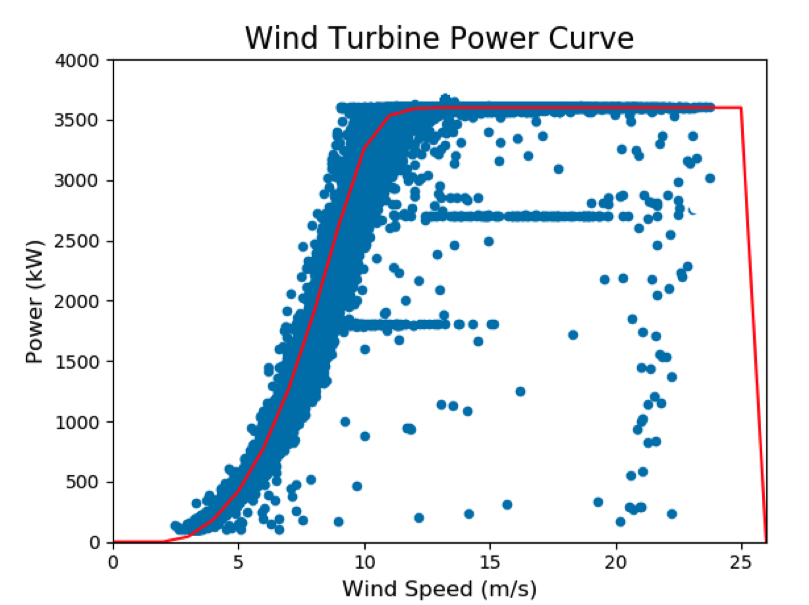
\includegraphics[width=0.6\textwidth]{figures/wind_power_curve.jpg}
\caption{"Power-Wind speed" curve of turbine \cite{Sofia}. Each blue dots represents a 10-minutes SCADA data point, red line is the theoretical power curve}
\label{fig:B-B1}
\end{figure}

\item \textbf{Data normalization}: Scale all the variables to the same range to eliminate the scale effect. The following formula is used:

$$x' = \frac{x-mean(x)}{std(x)}$$

where $mean(x)$ is the average value of variable $x$, $std(x)$ is standard deviation of variable $x$.

\end{enumerate}

\subsection{Model development}
Figure 7 shows general steps to build neural networks.

\begin{figure}[]
\centering
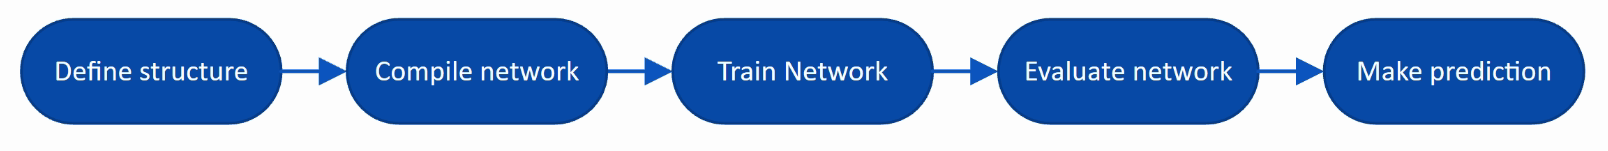
\includegraphics[width=0.8\textwidth]{figures/visio.png}
\caption{General steps to build neural networks}
\label{fig:B-B1}
\end{figure}

\subsubsection{Define structure}
The first step is to decide the type of the neural network. Then the detailed structure parameters should be defined. Activation function should also be defined if necessary.

\subsubsection{Compile network}
The second step is to arrange the sequence of layers. The network will be trained and evaluated through a series of matrix transforms. Furthermore, the optimization algorithm and loss function need to be defined in this step. Detailed introduction on optimization algorithm is shown in Appendix B. For this study, a Adaptive Moment Estimation (Adam) algorithm was used for the optimization.

\subsubsection{Train Network}
Training set has already been defined in data pre-processing section. Training set is used to update the weights of neurons to create a good mapping of inputs to outputs, and an optimization algorithm is also involved here. In this step, epoch number and batch size are defined.

The number of epoch determines how many times the optimization algorithm will work through the entire training set during the training process. Too few epochs will result in an under-fitted model while too many epochs will lead to an over-fitted model. Both of them produce inaccurate result when presented with new data.

The batch size is the number of training examples utilized in one iteration. Grid search algorithm can be used here to find an optimal value of batch size. The maximum value of batch size is also limited by the available memory of computer.

\subsubsection{Evaluate network}
In this step, the network was evaluated on the evaluation set, to test its performance on unseen data. Usually evaluation set is part of training set. After evaluation process, training set is combined with evaluation set to form a complete training set. Network are trained again on this larger training set.

\section{Regression Model}
It's natural to start with developing a simple regression model of unsupervised approach. One simple regression model was an ANN with one fully connected hidden layer containing 10 neurons \cite{Sofia}. The output is continuous numeric value. Then the health status is decided based on the difference between predicted values and real values. The majority of works on regression model use traditional ANN and RNN, but few of them use LSTM which have better performance on time series data. In this section, we tried to substitute the simple fully connected neural network with the LSTM network.

\subsection{Data Pre-processing}
In addition to the general data pre-processing steps, some extra data pre-processing steps also need to be done to make data suitable for our LSTM-based regression model. 

\begin{enumerate}
\item \textbf{Variables selection}

Input and output variables selections are mainly based on the type of failure. As for a gearbox failure, we can choose certain gearbox component as output variable (target variables)\cite{kusiak2011prediction}, and related environmental variables as input variables. In this case, our goal is to build model to predict gearbox failure. And we used the following choice shown in table 3.  

\begin{table}[]
\centering
\begin{tabular}{|c|c|}
\hline
\textbf{Input Variables} & \textbf{Output Variables} \\ \hline
Power                    & gear oil temperature      \\ \hline
Wind Speed               &                           \\ \hline
Ambient Temperature      &                           \\ \hline
gear oil temperature     &                           \\ \hline
High speed bearing temperature  &                    \\ \hline
\end{tabular}
\caption{Variables selection}
\end{table}

Note that the autoregressive model was used here, where historical values of the target variable were used to build the model and predict the target output\cite{tautz2016using}.

\item \textbf{Data windowing}

The regression models make a set of predictions based on a window of consecutive samples from the data. The main feature of the input windows need to be decided is the width (number of time steps) of the input and label windows. For example, to make a prediction of output variable 1 step (10 minutes) into the future, given 120 steps (20 hours) of history of input variables, a window should be defined like this:

\begin{figure}[]
\centering
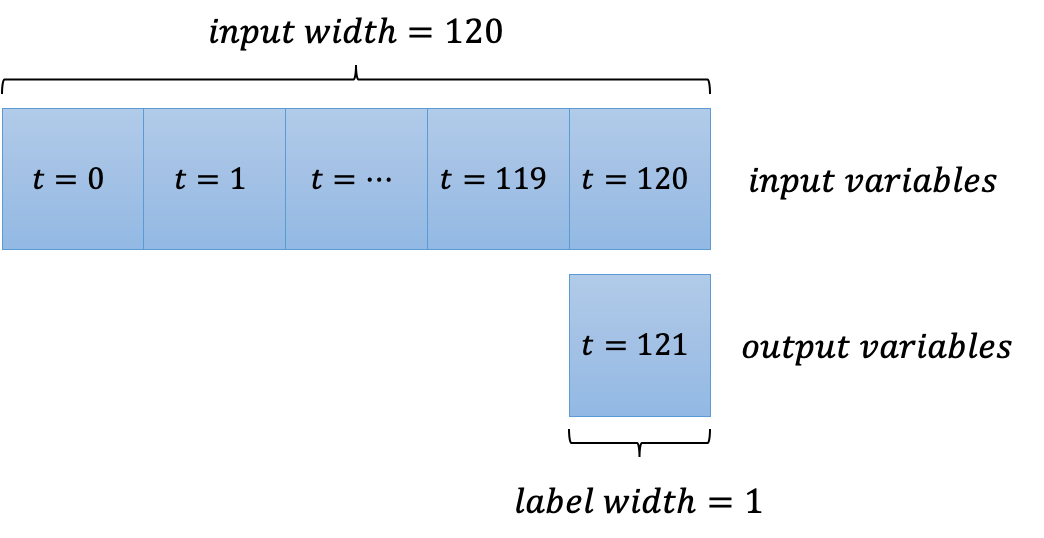
\includegraphics[width=0.7\textwidth]{figures/datawindow.png}
\caption{The window of input data}
\label{fig:B-B1}
\end{figure}

\item \textbf{Data set division}

For training and validating the model, the data set was divided into three parts, training set, validation set and test set. Since the objective of regression model is to predict target variables' value of normal operating state, one year data whose end date is 3 months ahead of failure occurrence was chosen as the training period set. Then the training period data set was randomly split into a training set (80\% of data set) and a testing set (20\% of data set). From 3 months ahead of failure occurrence to the point of failure occurrence, data of abnormal state was chosen as the test set.

\end{enumerate}

\subsection{Model Development}
The keras library provide simple implementation of LSTM model. By setting the "return\_sequence" as false and a proper batch size, a LSTM model is completely built. And the procedure of training and evaluating the model has been demonstrated in previous section.

\subsection{Result and Discussion}

\begin{figure}[]
\centering
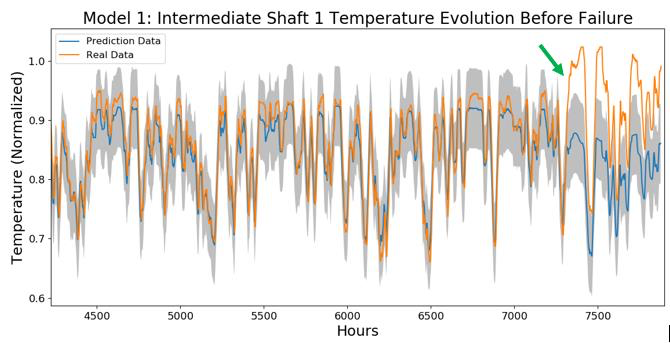
\includegraphics[width=0.9\textwidth]{figures/sofia_temp.png}
\caption{Intermediate shaft 1 temperature evolution \cite{Sofia}. Blue line: predicted temperature evolution, orange line: real temperature evolution. Grey region represents the prediction interval.}
\label{fig:B-B1}
\end{figure}

\begin{figure}[]
\centering
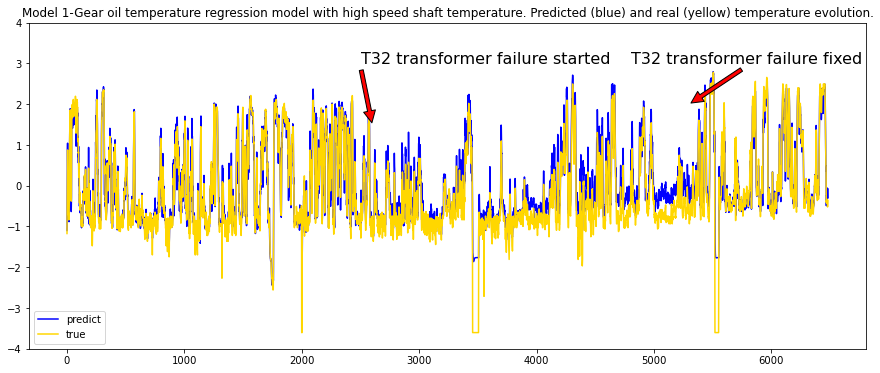
\includegraphics[width=0.9\textwidth]{figures/regression.png}
\caption{Gear oil temperature evolution during turbine LLY-21 failure development. Blue line: predicted temperature evolution, yellow line: real temperature evolution. Red arrows represent important events of failures}
\label{fig:B-B1}
\end{figure}

It can be seen from figure 9 that the predicted values exactly follow the fluctuations of the real values. This means that the LSTM-based regression model is able to extract the underlying time-related information of SCADA data. There is a considerably deviation between predicted values and real values in the time interval indicated by two red arrows. This means that the regression model was able to predict the incipient failure approximately 3000 hours before it was detected by the other monitoring system.

However, a target variable which has direct relation with the failure is required for this method (e.g. gear oil temperature in this case). The incipient component failures should have obvious influence on the value of this variable. Following a regression model\cite{Sofia}, intermediate shaft 1 temperature was used as output variable to predict the gearbox failure. Figure 9 shows that there is a significant increase of this value before the occurrence of failure. In this project, only two variables related to gearbox failure were provided. It is a common problem that a failure can not be represented by one variables. To address this issue, a different strategy need to be developed to make use of all available variables.


\section{Binary Classification Model}
With the consideration of limited SCADA variables, supervised approaches which do not require a direct failure related variable was developed. 

\subsection{Data Pre-processing}

\begin{enumerate}
\item \textbf{Variables selection}
This binary classification model does not require a direct failure related variable, so that all environmental variables (e.g. wind speed, ambient temperature) and state variables (e.g. gear oil temperature, generator temperature) can be used as inputs. In this case, in order to predict a failure, three environmental variables (wind speed, ambient temperature) and three state variables (power, gear oil temperature and high speed bearing temperature) were selected.

\item \textbf{Labels definition}
Labels representing two classes are required for the binary classification model. Data points which are 5 months ahead of failure occurrence were labeled with "0" while the rest data points which close to the failure occurrence were labeled with "1". 

\item \textbf{Data set division}
All data points were randomly split into a training set (80\% of data set) and a testing set (20\% of data set).

\end{enumerate}

\subsection{Model Development}
A simple ANN with two fully connected hidden layers was built as a classifier. There are 100 neurons in the first hidden layer, 50 neurons in the second hidden layer. The values of these two hyper-parameters are carefully chose to achieve good performance on detecting highly non-linear relationships in data with low computational cost. The output layer contains 2 neurons because the label contains two classes. ReLU function was chosen as the activation function. And logsoftmax function was used in the output layer, as one hot-encoding was used to define each class. With these numerical outputs, the prediction accuracy is defined as the number of correctly predicted states divided by the number of all outputs for a testing period.

\subsection{Result and Discussion}

\begin{figure}[]
\centering
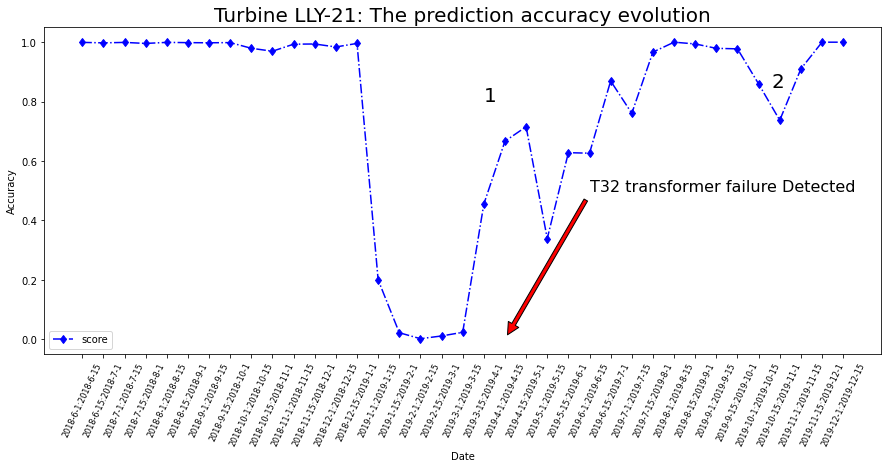
\includegraphics[width=0.9\textwidth]{figures/LLY21_binary.png}
\caption{Turbine LLY21-Binary classification model. Prediction accuracy (blue line) evolution from 2018-6 to 2019-12.}
\label{fig:B-B1}
\end{figure}

According to the status record, "T32 transformer failure" was detected on 24-Sep-2019. In addition to component failure, several maintenance was also recorded. They were supposed to be preventive measure to avoid failures. Details are shown in table 4.

\begin{table}[]
\centering
\begin{tabular}{|c|c|c|}
\hline
\textbf{Categories}                                            & \textbf{Failure and maintenance} & \textbf{Start data} \\ \hline
Failure                                                        & T32 transformer failure          & 2019-07-24          \\ \hline
\begin{tabular}[c]{@{}c@{}}Preventive\\ maintence\end{tabular} & TX replacement (T17)             & 2018-06-28          \\ \hline
                                                               & TX replacement (T25)             & 2018-09-24          \\ \hline
                                                               & Gear oil change                  & 2018-10-10          \\ \hline
                                                               & TX replacement (T26)             & 2019-01-09          \\ \hline
                                                               & T16 transformer exchange         & 2019-09-24          \\ \hline
                                                               & Gear oil cold or superheated     & 2019-12-16          \\ \hline
\end{tabular}
\caption{Status record of wind turbine LLY-21 (2018.06.01-2019.12.30)}
\end{table}



It can be seen from the figure 11 that the huge trough 1 corresponds to "T32 transformer failure" and trough 2 corresponds to "Gear oil problems". However, there were two recorded maintenance carried out in the flat part of the blue line which corresponds to training data set. The model obviously ignore these events. This can be explained by the model over-fitting. Since there were not enough related variables (e.g. bearing temperature corresponds to gearbox failure), the model was easily over-fitted during training process.

In addition, the binary classification model simple used all selected variables without considering the underlying relationship environmental variables and status variables. More features of the data need to be extracted before the training process. 

\section{Advanced Multinomial Classification Model}
An advanced multinomial classification model was developed to address the issues mentioned above. In order to avoid over-fitting, the model was designed to be general failure predictor which was not purpose-designed for specific failure.

\subsection{Data Pre-processing}

\begin{enumerate}
\item \textbf{Variables selection}
Two environmental variables and all four failure-related variables were selected even though they were related to different types of failures.

\begin{itemize}
\item Ambient Temperature
\item Power
\item Gear oil temperature
\item Generator RPM
\item Generator temperature
\item High speed bearing temperature
\end{itemize}

\item \textbf{Division of operating state}
Cui et al \cite{cui2018anomaly} introduced a method of removing outliers in SCADA data. The data were separated into clusters based on the wind speed and production power. Points which located outside three standard deviations from the mean value in each cluster by Mahalanobis distance were assumed to be outliers and were deleted by the filter. With the consideration of this, variables above were divided into two groups, "active variables" and "passive variables". Active variables include ambient temperature, power and wind speed while passive variables include gear oil temperature, generator RPM, generator temperature and high speed bearing temperature. Then data were separated into clusters based on three active variables. Each cluster represented an operating state. Once the values of active variables and the operating states were given, the range of passive variables' values would be fixed. In this case, operating state of the turbine is divided into 8 classes according to three active variables. Each class of operating state was labeled with a number from 0 to 7.

\begin{figure}[]
\centering
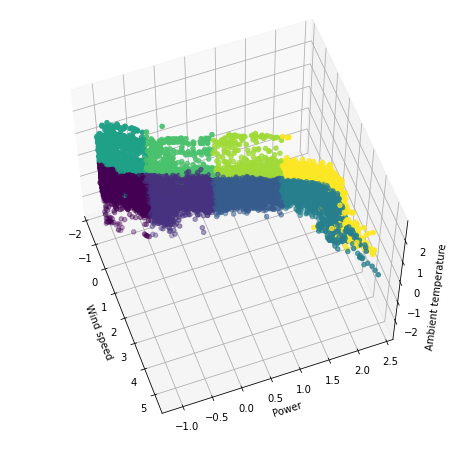
\includegraphics[width=0.59\textwidth]{figures/operating_state_division3d.png}
\caption{Division of operating state. Each cluster with certain color represents one operating state. The values of three variables are normalized values.}
\label{fig:B-B1}
\end{figure}

\item \textbf{Data set division}
All data points were randomly split into a training set (80\% of data set) and a testing set (20\% of data set).

\end{enumerate}

\subsection{Model development}
As mentioned above, operating states have direct relation with passive variables. Given values of passive variables, their operating states can also be predicted. A multinomial classification model was developed here to do this job.

\subsubsection{Define structure}
In this case, a simple neural network with two fully connected hidden layers was designed. There are 100 neurons in the first hidden layer, 50 neurons in the second hidden layer. The number of neurons in the input layer equals to the number of input variables which is 4. Since there are 8 different operating states, the output layer contains 8 neurons. The number of neurons was chosen through trial and two hidden layers were used to reduce the training complexity of the models. ReLU function was chosen as the activation function and logsoftmax function was used in the output layer to produce one-hot-encoding result.

\subsubsection{Make prediction}
After the training and evaluation process, predictions are made by introducing pre-processed test data set. Using the logsoftmax function, a probability result was given by the models. In this case, the largest one represented the operating state the corresponding turbine at this time point belongs to. Given one data point as input, the final output of this model will be a number which represents the corresponding operating state.

\subsubsection{Decide health state}
With these numerical outputs, the prediction accuracy, defined as the number of correctly predicted states divided by the number of all outputs for a testing period, can be regards as the "health score" of the wind turbine.

As shown in figure 13, the average accuracy score of training period is higher than 0.75. Since all the data points in training period is supposed to be at normal operating state, so that score higher than "0.75" represents state "OK". Since the lowest accuracy score is close to 0, it is natural to define "0.5-0.75" as "Monitor", "0.25-0.5" as "Inspect" and "0.0-0.25" as "Replace".

\subsection{Result and Discussion}

\subsubsection{Wind turbine LLY-21}

\begin{table}[]
\centering
\begin{tabular}{|c|c|c|}
\hline
\textbf{Categories}                                            & \textbf{Failure and maintenance}        & \textbf{Start data} \\ \hline
Failure                                                        & T32 transformer failure                 & 2019-07-24          \\ \hline
                                                               & Damage to bearings in gearbox           & 2020-02-06          \\ \hline
\begin{tabular}[c]{@{}c@{}}Preventive\\ maintence\end{tabular} & T07 transformer replacement             & 2019-06-20          \\ \hline
                                                               & T16 transformer exchange                & 2019-09-24          \\ \hline
                                                               & Gearbox oil cooler hose replacement     & 2020-01-09          \\ \hline
\end{tabular}
\caption{Status record of wind turbine LLY-12 (2019.06.01-2020.05.15)}
\end{table}

\begin{figure}[]
\centering
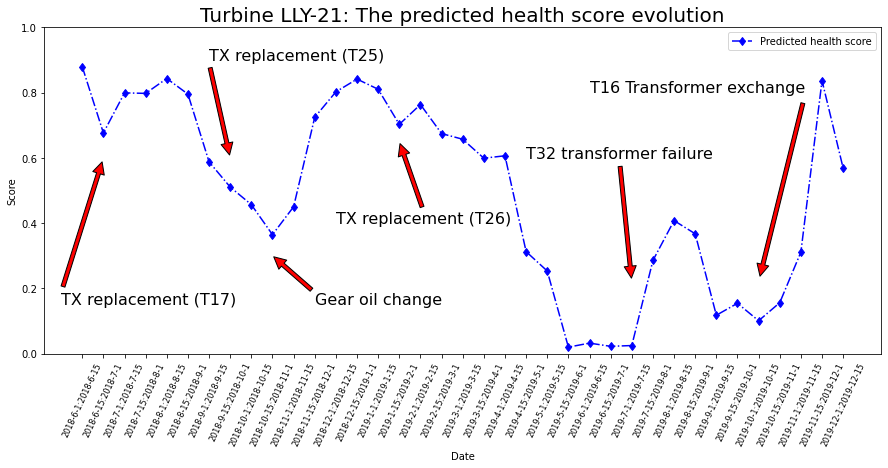
\includegraphics[width=0.9\textwidth]{figures/LLY21_multi.png}
\caption{Turbine LLY21-Advanced multinomial classification model. Predicted health score (blue line) evolution from 2018-6 to 2019-12.}
\label{fig:B-B1}
\end{figure}

\begin{figure}[]
\centering
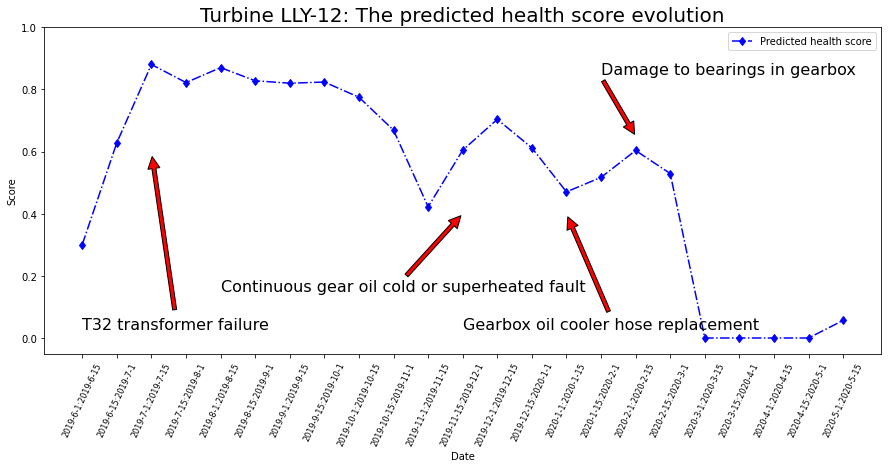
\includegraphics[width=0.9\textwidth]{figures/LLY12_multi.png}
\caption{Turbine LLY12-Advanced multinomial classification model. Predicted health score (blue line) evolution from 2019-1 to 2020-5.}
\label{fig:B-B1}
\end{figure}

Figure 13 and 14 show the sliding windows of the health score evolution of two turbines. Each trough represents an anomaly alarm which corresponds to an incipient failure. Slopes represent the growth of the failure. Serious failure (e.g. T32 transformer failure) leads to very low health score and "Replace" alarm was triggered. The other alarms can be explained as early stage failures and the growth of these failures were stopped by preventive maintenance.

All abnormal states of turbine LLT-21 were detected by this model according to health score evolution graph (figure 11) and status record (table 4). In terms of the major serious transformer failure of LLY-21, there is a "Replace" alarm triggered more than 2 months before the outage. Early stage failures are also detected by this model. Turning now to turbine LLY-12, it can be seen from figure 12 that the model ignored some failures. This is because this model is not expected to detect all types of failures with the consideration of limited input variables. Even so, this model is able to detect major failures listed in table 5.

Since this advanced multinomial classification model is not purpose-designed for specific failure, the health score is influenced by different types of failures which makes it hard for users to find out which failure the alarm corresponds to. However, given enough SCADA variables, this model can be easily changed to be a purpose-designed model for specific failure. 